\documentclass[a4paper,11pt]{exam}
\printanswers % pour imprimer les réponses (corrigé)
%\noprintanswers % Pour ne pas imprimer les réponses (énoncé)
\addpoints % Pour compter les points
% \noaddpoints % pour ne pas compter les points
%\qformat{\textbf{\thequestion ) } }
\qformat{\textbf{\thequestion )}} % Pour définir le style des questions (facultatif)
\usepackage{color} % définit une nouvelle couleur
\shadedsolutions % définit le style des réponses
% \framedsolutions % définit le style des réponses
\definecolor{SolutionColor}{rgb}{0.8,0.9,1} % bleu ciel
\renewcommand{\solutiontitle}{\noindent\textbf{Solution:}\par\noindent} % Définit le titre des solutions




\makeatletter

\def\maketitle{{\centering%
	\par{\huge\textbf{\@title}}%
	\par{\@date}%
	\par}}


\renewcommand{\thesubsection}{\Alph{subsection}.}   

\makeatother

\lhead{NOM Pr\'enom :}
\rhead{\textbf{Les r\'eponses doivent \^etre justifi\'ees et r\'edig\'ees}}
\cfoot{\thepage / \pageref{LastPage}}


%\usepackage{../../pas-math}
%\usepackage{../../moncours}


%\usepackage{pas-cours}
%-------------------------------------------------------------------------------
%          -Packages nécessaires pour écrire en Français et en UTF8-
%-------------------------------------------------------------------------------
\usepackage[utf8]{inputenc}
\usepackage[frenchb]{babel}
%\usepackage{numprint}
\usepackage[T1]{fontenc}
%\usepackage{lmodern}
\usepackage{textcomp}
\usepackage[french, boxed]{algorithm2e}
\usepackage{hyperref}


%-------------------------------------------------------------------------------

%-------------------------------------------------------------------------------
%                          -Outils de mise en forme-
%-------------------------------------------------------------------------------
\usepackage{hyperref}
\hypersetup{pdfstartview=XYZ}
%\usepackage{enumerate}
\usepackage{graphicx}
\usepackage{multicol}
\usepackage{tabularx}
\usepackage{multirow}
\usepackage{color}
\usepackage{eurosym}


\usepackage{anysize} %%pour pouvoir mettre les marges qu'on veut
%\marginsize{2.5cm}{2.5cm}{2.5cm}{2.5cm}

\usepackage{indentfirst} %%pour que les premier paragraphes soient aussi indentés
\usepackage{verbatim}
\usepackage{enumitem}
\usepackage{booktabs}
\usepackage[usenames,dvipsnames,svgnames,table]{xcolor}

\usepackage{variations}

%-------------------------------------------------------------------------------


%-------------------------------------------------------------------------------
%                  -Nécessaires pour écrire des mathématiques-
%-------------------------------------------------------------------------------
\usepackage{amsfonts}
\usepackage{amssymb}
\usepackage{amsmath}
\usepackage{amsthm}
\usepackage{tikz}
\usepackage{xlop}
\usepackage[output-decimal-marker={,}]{siunitx}
%-------------------------------------------------------------------------------

%-------------------------------------------------------------------------------
%                  -Nécessaires pour écrire des formules chimiquess-
%-------------------------------------------------------------------------------

\usepackage[version=4]{mhchem}

%-------------------------------------------------------------------------------
% Pour pouvoir exploiter les fichiers directement dans beamer
\newcommand{\pause}{\ }
%-------------------------------------------------------------------------------
%                    - Mise en forme avancée
%-------------------------------------------------------------------------------

\usepackage{ifthen}
\usepackage{ifmtarg}


\newcommand{\ifTrue}[2]{\ifthenelse{\equal{#1}{true}}{#2}{$\qquad \qquad$}}

%\newcommand{\kword}[1]{\textcolor{red}{\underline{#1}}}
%-------------------------------------------------------------------------------

%-------------------------------------------------------------------------------
%                     -Mise en forme d'exercices-
%-------------------------------------------------------------------------------
%\newtheoremstyle{exostyle}
%{\topsep}% espace avant
%{\topsep}% espace apres
%{}% Police utilisee par le style de thm
%{}% Indentation (vide = aucune, \parindent = indentation paragraphe)
%{\bfseries}% Police du titre de thm
%{.}% Signe de ponctuation apres le titre du thm
%{ }% Espace apres le titre du thm (\newline = linebreak)
%{\thmname{#1}\thmnumber{ #2}\thmnote{. \normalfont{\textit{#3}}}}% composants du titre du thm : \thmname = nom du thm, \thmnumber = numéro du thm, \thmnote = sous-titre du thm

%\theoremstyle{exostyle}
%\newtheorem{exercice}{Exercice}
%
%\newenvironment{questions}{
%\begin{enumerate}[\hspace{12pt}\bfseries\itshape a.]}{\end{enumerate}
%} %mettre un 1 à la place du a si on veut des numéros au lieu de lettres pour les questions 
%-------------------------------------------------------------------------------

%-------------------------------------------------------------------------------
%                    - Mise en forme de tableaux -
%-------------------------------------------------------------------------------

\renewcommand{\arraystretch}{1.7}

\setlength{\tabcolsep}{1.2cm}

%-------------------------------------------------------------------------------



%-------------------------------------------------------------------------------
%                    - Racourcis d'écriture -
%-------------------------------------------------------------------------------
%Droites
\newcommand{\dte}[1]{$(#1)$}
\newcommand{\fig}[1]{figure $#1$}
\newcommand{\sym}{symétrique}
\newcommand{\syms}{symétriques}
\newcommand{\asym}{axe de symétrie}
\newcommand{\asyms}{axes de symétrie}
\newcommand{\seg}[1]{$[#1]$}
\newcommand{\monAngle}[1]{$\widehat{#1}$}
\newcommand{\bissec}{bissectrice}
\newcommand{\mediat}{médiatrice}
\newcommand{\ddte}[1]{$[#1)$}


% Angles orientés (couples de vecteurs)
\newcommand{\aopp}[2]{(\vec{#1}, \vec{#2})} %Les deuc vecteurs sont positifs
\newcommand{\aopn}[2]{(\vec{#1}, -\vec{#2})} %Le second vecteur est négatif
\newcommand{\aonp}[2]{(-\vec{#1}, \vec{#2})} %Le premier vecteur est négatif
\newcommand{\aonn}[2]{(-\vec{#1}, -\vec{#2})} %Les deux vecteurs sont négatifs

%Ensembles mathématiques
\newcommand{\naturels}{\mathbb{N}} %Nombres naturels
\newcommand{\relatifs}{\mathbb{Z}} %Nombres relatifs
\newcommand{\rationnels}{\mathbb{Q}} %Nombres rationnels
\newcommand{\reels}{\mathbb{R}} %Nombres réels
\newcommand{\complexes}{\mathbb{C}} %Nombres complexes


%Intégration des parenthèses aux cosinus
\newcommand{\cosP}[1]{\cos\left(#1\right)}
\newcommand{\sinP}[1]{\sin\left(#1\right)}


%Probas stats
\newcommand{\stat}{statistique}
\newcommand{\stats}{statistiques}


\newcommand{\homo}{homothétie}
\newcommand{\homos}{homothéties}


\newcommand{\mycoord}[3]{(\textcolor{red}{\num{#1}} ; \textcolor{Green}{\num{#2}} ; \textcolor{blue}{\num{#3}})}
%-------------------------------------------------------------------------------

%-------------------------------------------------------------------------------
%                    - Mise en page -
%-------------------------------------------------------------------------------

\newcommand{\twoCol}[1]{\begin{multicols}{2}#1\end{multicols}}


\setenumerate[1]{font=\bfseries,label=\textit{\alph*})}
\setenumerate[2]{font=\bfseries,label=\arabic*)}


%-------------------------------------------------------------------------------
%                    - Elements cours -
%-------------------------------------------------------------------------------

%Correction d'exercice
\newcommand{\exoSec}[2]{\subsection*{Exercice #1 page #2}}
%-------------------------------------------------------------------------------
%                    - raccourcis d'écriture -
%-------------------------------------------------------------------------------

%Mise en évidence de termes clés
\newcommand{\mykw}[1]{\textcolor{red}{\underline{\textbf{#1}}}}

%Exercices
\newcommand{\exo}[2]{exercice #1 page #2}
\newcommand{\Exo}[2]{Exercice #1 page #2}

\renewcommand{\pause}{\ }

%Intervalles
\newcommand{\interOO}[2]{$]$#1 , #2$[$}
\newcommand{\interOF}[2]{$]$#1 , #2$]$}
\newcommand{\interFO}[2]{$[$#1 , #2$[$}
\newcommand{\interFF}[2]{$[$#1 , #2$]$}



%\usepackage{fullpage}
\author{\ }
\date{18 Décembre 2017}
\title{Sciences Physiques : DS n° 3}


\begin{document}
%	\usepackage{fancyhdr}
%	
%	\pagestyle{fancy}
%	\fancyhf{}
	%\rhead{Share\LaTeX}

	\maketitle
	
	

%\vspace*{-0.5cm}	

%\begin{small}
%	\begin{center}
%		\begin{tabular}{|@{\ }l@{}|@{\ }c@{\ }|}
%			\hline
%			\textbf{Compétence} & \textbf{Maitrise} \\
%			\hline
%			Conservation de la masse, variation du volume, température de changement d’état &  \ \ \ \\
%			\hline
%			Mettre en oeuvre des tests caractéristiques d’espèces chimiques à partir d’une banque fournie. &  \\
%			\hline			
%		\end{tabular}
%	\end{center}
%\end{small}	

\section{Différencier deux produits}

Lola doit étiqueter deux tubes à essais. L'un contient de l'eau, l'autre du cyclohexane. Elle sait que le cyclohexane ne contient pas d'eau mais est également transparent.

\begin{questions}
	\question Comment peut-elle faire pour mettre les bonnes étiquettes sur les bons tubes ? Expliquez votre \underline{argumentation} et faites un \underline{schéma}.
	
	\begin{solution}
		Pour identifier chaque tube, on utilise du sulfate de cuivre anhydre. Dans une boite de petri on dispose du sulfate de cuivre anhydre. On choisi ensuite un tube à essais puis on verse quelques goutes du liquide qu'il contient sur le sulfate de cuivre anhydre. Si le sulfate de cuivre devient bleu, ce tube contient de l'eau et donc l'autre contient du cyclohéxane. S'il reste blanc, le tube choisi contient du cyclohéxane et l'autre de l'eau.
	\end{solution}
\end{questions}


\section{Repas de midi}

A leur repas de midi, Manon et Jade ont mangé 140 g de pâtes, un steak haché de 125 g, un verre de lait (25 cL) et une pomme (85 g).


\begin{questions}
	\question Calculer la quantité d'eau absorbée par chacune au cours du repas en utilisant le tableau ci-dessous. (Faire apparaître tous vos calculs)
	\begin{solution}
		\begin{itemize}
			\item Calcul de la quantité d'eau dans 140 g de pâtes :
			\begin{equation*}
				\frac{200}{100}= \num{2}
			\end{equation*}
			1g de pâtes cuites contient \num{2} mL d'eau.
			\begin{equation*}
			\num{2} \times 140 = 280
			\end{equation*}
			140 g de pâtes cuites contiennent 280 mL d'eau.
			
			
			\item Calcul de la quantité d'eau dans un steak haché  de 125 g :
			\begin{equation*}
			\frac{84}{100}= \num{0.84}
			\end{equation*}
			1g de steak haché contient \num{0.84} mL d'eau.
			\begin{equation*}
			\num{0.84} \times 125 = 105
			\end{equation*}
			Un steak haché de 125 g contient 105 mL d'eau.
			
			\item Calcul de la quantité d'eau dans 25 cL de lait :
			\begin{equation*}
			\frac{84}{100}= \num{0.84}
			\end{equation*}
			1 mL de lait contient \num{0.84} mL d'eau.
			
			$25 cL = 250 mL$
			\begin{equation*}
			\num{0.84} \times 250 = \num{202.5}
			\end{equation*}
			25 cL de lait contiennent \num{202.5} mL d'eau.
			
			\item Calcul de la quantité d'eau dans une pomme de 85 g :
			\begin{equation*}
			\frac{70}{100}= \num{0.7}
			\end{equation*}
			1g de pomme contient \num{0.7} mL d'eau.
			\begin{equation*}
			\num{0.7} \times 85 = \num{59.5}
			\end{equation*}
			Une pomme de 85 g contient \num{59.5} mL d'eau.
			
			\item Total
			\begin{equation*}
				280 + 105 + \num{202.5} + \num{59.5} = 647
			\end{equation*}
			
			Au cours du repas, Manon et Jade ont absorbé 647 mL d'eau.
		\end{itemize}
	
	\end{solution}
	
	\question Marion n'a pas voulu son verre de lait mais a mangé deux pommes (de 85 g) et bu un verre et demi d'eau (1 verre = 120 ml). A-t-elle absorbée plus d'eau que Manon et Jade ? ((Faire apparaître tous vos calculs))
	
	\begin{solution}
		\begin{itemize}
			\item Calcul de la quantité d'eau contenue dans deux pommes de 85 g chacune :
			Une pomme de 85 g contient \num{59.5} mL d'eau, donc deux pommes contiennent 119 mL d'eau ($\num{59.5} \times 2$).
			
			
			\item Total :
			Marion a mangé 140 g de pâtes cuites (280 mL), un steak haché de 125 g (105 mL), deux pommes (119 mL) et a bu un verre d'eau et demi ($120 \times \num{1.5} = 180 g$).
			
			\begin{equation*}
				280 + 105 + 119 + 180 = 684
			\end{equation*}
			
			Au cours du repas, Marion a absorbé 684 mL d'eau, donc plus que Manon et Jade.
		\end{itemize}
	\end{solution}
\end{questions}

\begin{center}
	\begin{tabular}{|l|c|c|}
		\hline
		& Volume ou & Volume \\ 
		Aliment      & masse de  & d'eau  \\ 
		& l'aliment &        \\ \hline
		Lait entier  & 100 ml    & 81 mL  \\ \hline
		Pâtes cuites & 100 g     & 200 mL \\ \hline
		Pomme        & 100 g     & 70 mL  \\ \hline
		Steak haché  & 100 g     & 84 mL  \\ \hline
	\end{tabular}
\end{center}

%\newpage

\section{A l'encre bleue}

On a déposé quelques gouttes d'une encre bleue sur du sulfate de cuivre anhydre.

\begin{center}
	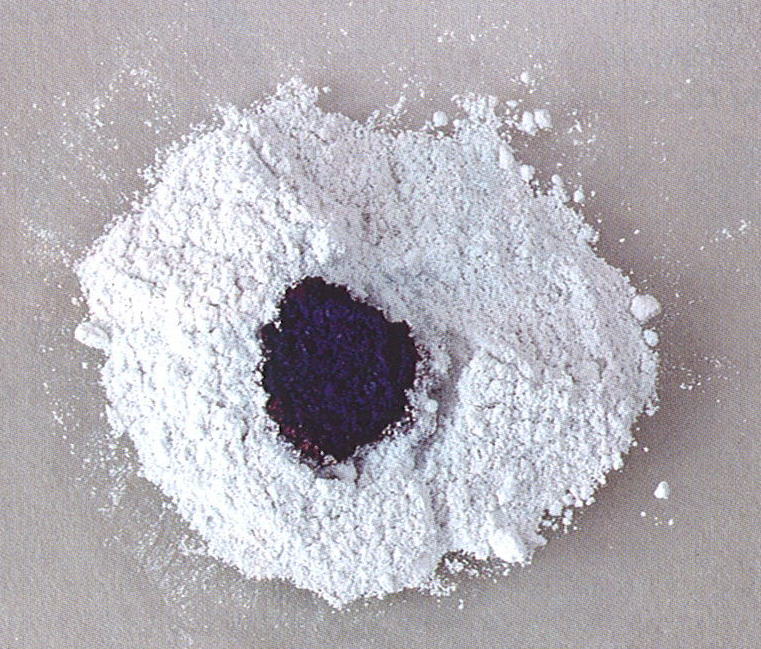
\includegraphics[scale=0.7]{encre}
\end{center}

\begin{questions}
	\question Cette expérience permet-elle de déterminer avec certitude si cette encre contient de l'eau ?
	\begin{solution}
		Le sulfate de cuivre anhydre, blanc, devient bleu en présence d'eau. Si on verse de l'encre bleue sur le sulfate de cuivre anhydre devient bleu à cause de la couleur de l'encre. Il n'est donc pas possible de voir s'il y a un changement de couleur à cause d'eau présente dans l'encre. J'en déduis qu'il n'est pas possible d'utiliser cette expérience pour déterminer avec certitude si l'encre contient de l'eau.
	\end{solution}
\end{questions}


\section{Le détecteur de l'eau}

On réalise le test caractéristique de l'eau dessiné ci-dessous.

\begin{center}
	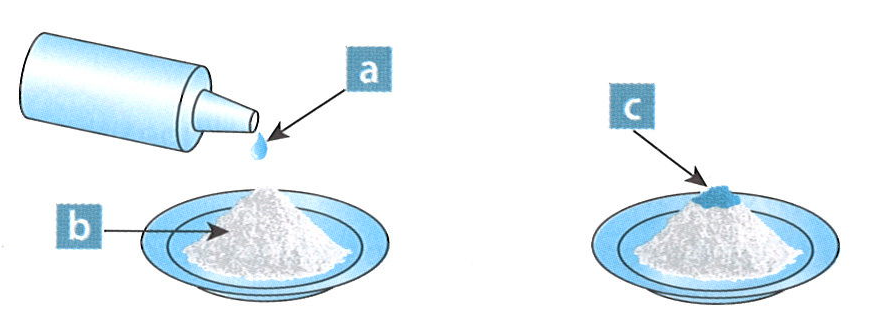
\includegraphics[scale=1]{schema}
\end{center}


\begin{questions}
	\question Attribuer à chaque lettre les mots ou groupes de mots suivants : \\
	eau - sulfate de cuivre hydraté - sulfate de cuivre anhydre.
	\begin{solution}
		\begin{enumerate}[label=\alph*.]
			\item eau ;
			\item sulfate de cuivre anhydre ;
			\item sulfate de cuivre hydraté.
		\end{enumerate}
	\end{solution}
\end{questions}


\ \label{LastPage}

\end{document}